\begin{figure}[H]
    \centering
    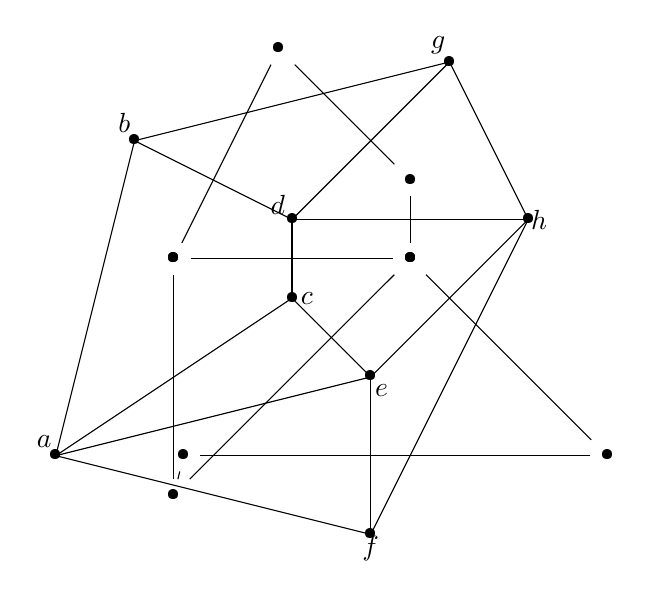
\begin{tikzpicture}
        \node[label={[label distance = -3mm]160:$a$}] at
        (-2.00, -1.00) {\textbullet};
        \node[label={[label distance = -3mm]160:$b$}] at
        (-1.00, 3.00) {\textbullet};
        \node[label={[label distance = -6mm]180:$c$}] at
        (1.00, 1.00) {\textbullet};
        \node[label={[label distance = -3mm]120:$d$}] at
        (1.00, 2.00) {\textbullet};
        \node[label={[label distance = -3mm]340:$e$}] at
        (2.00, 0.00) {\textbullet};
        \node[label={[label distance = -3mm]270:$f$}] at
        (2.00, -2.00) {\textbullet};
        \node[label={[label distance = -3mm]160:$g$}] at
        (3.00, 4.00) {\textbullet};
        \node[label={[label distance = -3mm]0:$h$}] at
        (4.00, 2.00) {\textbullet};

        \draw (-2.00, -1.00) -- (-1.00, 3.00); % a -- b
        \draw (-2.00, -1.00) -- (1.00, 1.00); % a -- c
        \draw (-2.00, -1.00) -- (2.00, 0.00); % a -- e
        \draw (-2.00, -1.00) -- (2.00, -2.00); % a -- f
%        \draw (-1.00, 3.00) -- (1.00, 1.00); % b -- c
        \draw (-1.00, 3.00) -- (1.00, 2.00); % b -- d
        \draw (-1.00, 3.00) -- (3.00, 4.00); % b -- g
        \draw (1.00, 1.00) -- (1.00, 2.00); % c -- d
        \draw (1.00, 1.00) -- (2.00, 0.00); % c -- e
%        \draw (1.00, 2.00) -- (2.00, 0.00); % d -- e
        \draw (1.00, 2.00) -- (3.00, 4.00); % d -- g
        \draw (1.00, 2.00) -- (4.00, 2.00); % d -- h
        \draw (2.00, 0.00) -- (2.00, -2.00); % e -- f
        \draw (2.00, 0.00) -- (4.00, 2.00); % e -- h
        \draw (2.00, -2.00) -- (4.00, 2.00); % f -- h
        \draw (3.00, 4.00) -- (4.00, 2.00); % g -- h

        \node (abc) at (-0.5, 1.5) {\textbullet}; % a-b-c
        \node (bcd) at (-0.5, 1.5) {\textbullet}; % b-c-d
        \node (bdg) at (0.8333333333333334, 4.166666666666667) {\textbullet}; % b-d-g
        \node (dhg) at (2.5, 2.5) {\textbullet}; % d-h-g
        \node (ced) at (2.5, 1.5) {\textbullet}; % c-e-d
        \node (deh) at (2.5, 1.5) {\textbullet}; % d-e-h
        \node (fhe) at (5.0, -1.0) {\textbullet}; % f-h-e
        \node (aec) at (-0.5, -1.5) {\textbullet}; % a-e-c
        \node (afe) at (-0.375, -1.0) {\textbullet}; % a-f-e
        
        \draw (abc) -- (aec);
        \draw (bcd) -- (bdg);
        \draw (bcd) -- (ced);
        \draw (bdg) -- (dhg);
        \draw (dhg) -- (deh);
        \draw (deh) -- (ced);
        \draw (deh) -- (fhe);
        \draw (fhe) -- (afe);
        \draw (afe) -- (aec);
        \draw (aec) -- (ced);


    \end{tikzpicture}
    \caption[Exemplo triangulação de Delaunay]{Exemplo.}\label{fig:delaunay:voronoi}
\end{figure}